%!TEX TS-program = pdflatex
%!TEX encoding = UTF-8 Unicode

\documentclass[11pt]{article}

\usepackage[utf8]{inputenc}
\usepackage{geometry}
\geometry{a4paper}
\usepackage{graphicx}
\usepackage{booktabs}
\usepackage{array}
\usepackage{verbatim}
\usepackage{subfig}
\usepackage{hyperref}

\usepackage{url}

\usepackage{fancyhdr} 
\pagestyle{fancy}
\renewcommand{\headrulewidth}{0pt} 
\lhead{}\chead{}\rhead{}
\lfoot{}\cfoot{\thepage}\rfoot{}

\usepackage{sectsty}
\allsectionsfont{\sffamily\mdseries\upshape}

\usepackage[nottoc,notlof,notlot]{tocbibind} 
\usepackage[titles,subfigure]{tocloft} 
\renewcommand{\cftsecfont}{\rmfamily\mdseries\upshape}
\renewcommand{\cftsecpagefont}{\rmfamily\mdseries\upshape}

\usepackage[spanish]{babel}
\usepackage{listings}

%%%El documento comienza aqui

\title{\textbf{Proyecto Parser XML - Python}}
\author{\textbf{Jimmy Banchón - Rene Balda}}
\date{\textbf{\today}}
\begin{document}

\bibliographystyle{plain}

\maketitle
\section{\textbf{Introducción}} 
\paragraph{} \noindent
El proyecto Parser XML se basa en leer un archivo XML y modelarlo en un objeto; mediante sus tags, usando funciones y construcciones basicas en el lenguaje {\textbf{Phyton}}.

Para este proyecto dispondremos del archivo {\textbf{wurfl-2.3.xml}}, el cuan consta de pocos niveles anidados para hacer mas facil y sencilla la implementacion de la lectura de tags. El lenguaje en el que se desarrollo este programa hace que los strings sean mas faciles de leer; por lo tanto es un lenguaje propicio para desarrollar programas que hagan este tipo de tareas.
\section{\textbf{Alcance del Proyecto}}

Nuestro proyecto cumplió con las siguientes características:
\begin{enumerate}
\item 
Lectura de todos los tags y atributos inherentes a éste.

\item
Cada tag esta representado por una clase, lo cual hace mas entendible su representacion en la estructura de datos.

\item
Funciones modularizadas.

\end{enumerate}
\paragraph{} \noindent De acuerdo a las características antes listadas se cree que se logro casi por completo todos los requetimientos designados para el desarrollo de este pequeño programa.

\section{Diagramación}


\subsection{\textbf{Diagrama de Clases}}

				\begin{center}
				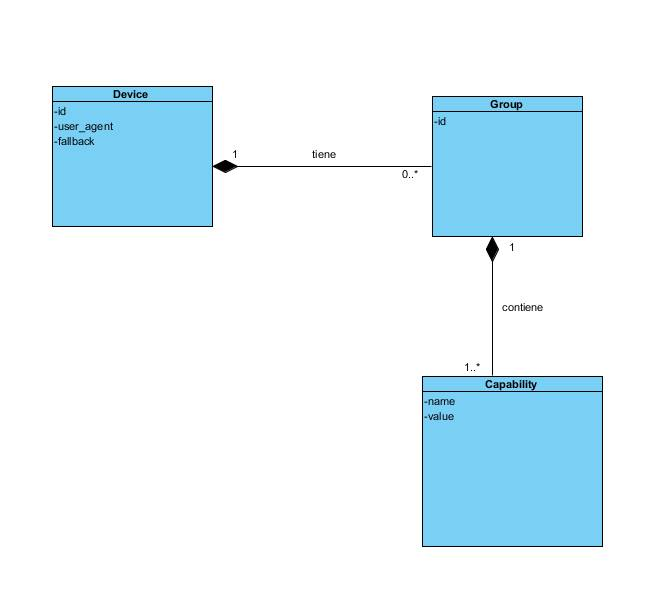
\includegraphics[width=0.71\textwidth]{images/class_diagram}
				\end{center}

\section{\textbf{Conclusiones}}
\begin{enumerate}
\item
{\textbf{Phyton}} es un lenguaje de programación que optimiza la manipulacion de Strings.
\item
El programa seria mucho mas dificil de mantener si los documentos a leer tuvieran muchos mas niveles anidados
\item
El lenguaje utilizado fue mucho mas facil de aprender y entender que cualquier otro que pertenezca al paradigma orientado a objetos.
\item
Existen diferencias de sintaxis entre Python 2.7 y Python 3.3

\end{enumerate}


\end{document}